% Uncomment this to make slides with overlays:
%\documentclass[slides]{beamer}

% Uncomment these (but comment the above \documentclass line) to make handouts:
\documentclass[handout]{beamer}

% Uncomment these to have more than one slide per page
%\usepackage{pgfpages}
%\pgfpagesuselayout{2 on 1}[border shrink=5mm]
%\pgfpageslogicalpageoptions{1}{border code=\pgfusepath{stroke}}
%\pgfpageslogicalpageoptions{2}{border code=\pgfusepath{stroke}}

\usepackage[]{graphicx, color, hyperref}

\mode<presentation>
{
	%\usetheme[secheader]{Boadilla}
	%\usecolortheme[rgb={.835, .102,.169}]{structure}  
	\usetheme[width= 0cm]{Goettingen}
	%\setbeamercovered{transparent}
}
\setbeamertemplate{navigation symbols}{}
\setbeamertemplate{footline}[frame number]

\definecolor{blue2}{rgb}{0.278,0.278,0.729} 
\newcommand{\blue}[1]{\textcolor{blue2}{#1}}
\newcommand{\white}[1]{\textcolor{white}{#1}}
\newcommand{\red}[1]{\textcolor{red}{#1}}
\newcommand{\xbar}{\overline{x}}
\newcommand{\ybar}{\overline{y}}
\newcommand{\phat}{\widehat{p}}
\newcommand{\prob}{\mbox{Pr}}
\newcommand{\E}{\mathbb{E}}
\newcommand{\Var}{\mbox{Var}}
\newcommand{\cp}{\oplus}
\newcommand{\cm}{\circleddash}

\title{Lecture 6: Examining/Visualizing Numerical Data Part 2}
\author{Chapter 1.6}
\date{}

\begin{document}
%------------------------------------------------------------------------------
\begin{frame}
\titlepage
\end{frame}
%------------------------------------------------------------------------------

%%------------------------------------------------------------------------------
%\begin{frame}
%\frametitle{Previously...}
%\begin{itemize}
%\item Showed two classic examples of data visualization:  Napoleon's advance/retreat on Moscow and John Snow's map of Cholera in London in 1854
%\item Reintroduced histograms
%\item Measures of central tendency: Mean, Median, Mode
%\item Measures of spread
%\end{itemize}
%
%\end{frame}
%%------------------------------------------------------------------------------
%
%
%%------------------------------------------------------------------------------
%\begin{frame}[fragile]
%\frametitle{Previously... Measure of Spread}
%
%Two related measures of \blue{spread/variability} are:
%\begin{itemize}
%\item The \blue{sample variance $s^2$} is roughly the average squared distance from the mean.
%\item The \blue{standard deviation $s = \sqrt{s^2}$} is the square root of the variance. The standard deviation is useful when considering how close the data are to the mean.
%\end{itemize}
%
%\end{frame}
%%------------------------------------------------------------------------------
%
%
%%------------------------------------------------------------------------------
%\begin{frame}[fragile]
%\frametitle{Previously... Measure of Spread}
%Back to example:
%\begin{center}
%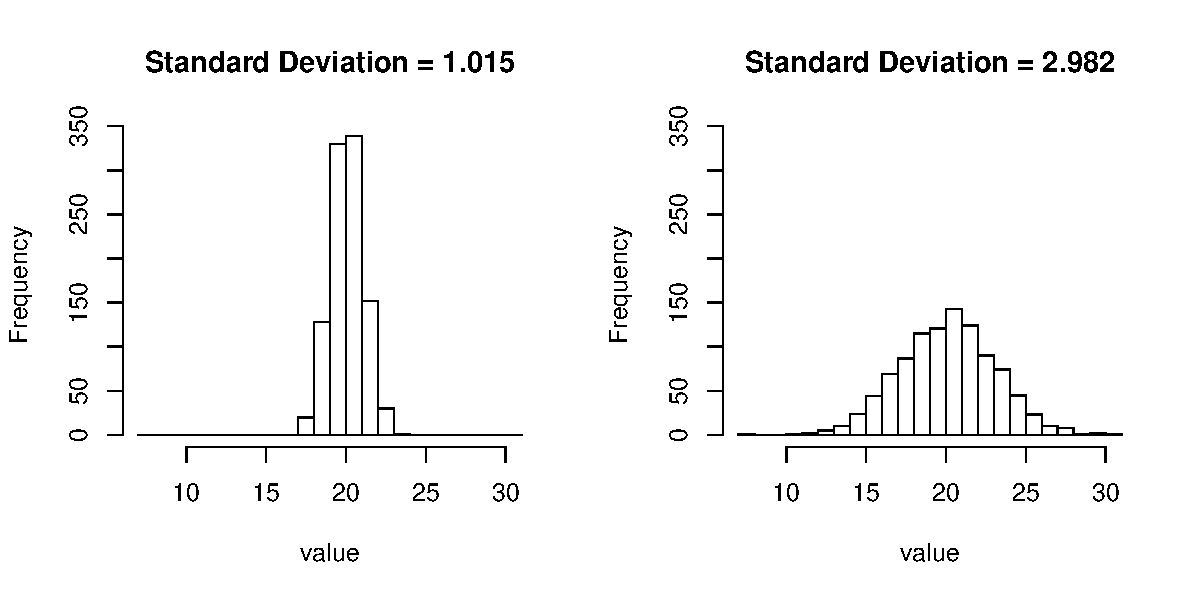
\includegraphics[width=\textwidth]{figure/spread2.pdf}
%\end{center}
%
%\end{frame}
%%------------------------------------------------------------------------------


%------------------------------------------------------------------------------
\begin{frame}[fragile]
\frametitle{Goals for Today}

\begin{itemize}
\item Rule of thumb for standard deviations
\item Population vs sample mean/variance/standard deviations
\item Percentiles and Quartiles
\item Boxplots
\end{itemize}

\end{frame}
%------------------------------------------------------------------------------


%------------------------------------------------------------------------------
\begin{frame}[fragile]
\frametitle{Rule of Thumb for Standard Deviations}

If the data distribution is bell-shaped, then about \blue{$\frac{2}{3}$'s of the data will be within one standard deviation of the mean} and about \blue{95\% will be within two standard deviations}.

\vspace{0.5cm}

\pause Notes:
\begin{itemize}
\pause\item The book has the first rule at 70\%, and not $\frac{2}{3}$'s.  
\pause\item This is not a hard and fast rule.  Look at examples in Figure 1.27 on page 27 of text.  
\end{itemize}

\end{frame}
%------------------------------------------------------------------------------


%------------------------------------------------------------------------------
\begin{frame}[fragile]
\frametitle{Going back to Second Example}

\begin{columns}
\column{.5\textwidth}
\begin{center}
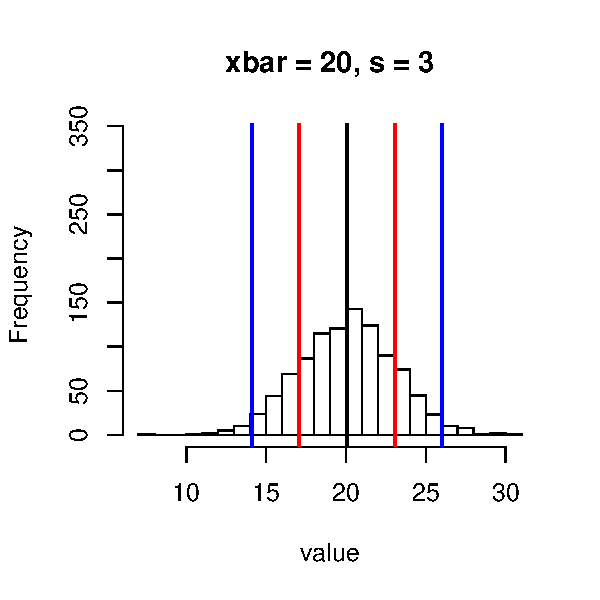
\includegraphics[width=\textwidth]{figure/spread3.pdf}
\end{center}
\column{.5\textwidth}
\pause Here
\begin{itemize}
\item black line is mean $\overline{x}$
\item red lines mark $[\overline{x} - s, \overline{x} + s] = [20 - 3, 20 + 3] = [17, 23]$
\item blue lines mark $[\overline{x} - 2s, \overline{x} + 2s] = [20 - 6, 20 + 6] = [14, 26]$
\end{itemize}
\end{columns}
\pause So roughly
\begin{itemize}
\item $\frac{2}{3}$'s of the data is between the red lines
\item 95\% of the data will is between the blue lines
\end{itemize}

\end{frame}
%------------------------------------------------------------------------------


%------------------------------------------------------------------------------
\begin{frame}[fragile]
\frametitle{Population vs Sample Mean/Variance/Standard Deviation}

Recall from Lecture 1.3 the notion of taking a \blue{sample} from a \blue{study/target population}:

\vspace{0.25cm}

\begin{center}
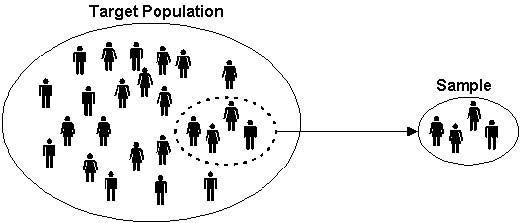
\includegraphics[width=3in]{figure/target-population.jpg} 
\end{center}

\vspace{0.25cm}

\pause We slowly start articulating this concept in statistical terms.  Say we are interested in the income of the individuals.   

\end{frame}
%------------------------------------------------------------------------------


%------------------------------------------------------------------------------
\begin{frame}[fragile]
\frametitle{Population vs Sample Mean/Variance/Standard Deviation}

The \blue{sample mean $\overline{x}$} is the mean income of the 4 individuals in our sample.  However, say we didn't just ask the 4 people in the sample for their income, but rather we asked all 24 individuals in the \blue{target population}.  \pause This mean would be the \blue{population mean $\mu$ (greek letter ``mu'')}.

\vspace{0.5cm}

\pause Much in the same vein:
\begin{itemize}
\item The \blue{sample variance $s^2$} is an estimator of the true population variance $\sigma^2$ (greek letter ``sigma'')
\pause \item The \blue{sample standard deviation $s$} is an estimator of the true population standard deviation $\sigma$
\end{itemize}



\end{frame}
%------------------------------------------------------------------------------


%------------------------------------------------------------------------------
\begin{frame}[fragile]
\frametitle{Population vs Sample Mean/Variance/Standard Deviation}

We say that the sample mean $\overline{x}$ is an \blue{estimator} of the \blue{true} population mean $\mu$ (remember the notion of \blue{generalizability}).  This will be the basis of future lectures based on Chapter 4 from the text.  

\vspace{0.5cm}

\pause In this example, 24 is a rather small number, so what's the real leap between between $\overline{x}$ and $\mu$?  Imagine instead your population is 300 million people!  Not so easy.  We need $\overline{x}$ to \blue{estimate} $\mu$.
\end{frame}
%------------------------------------------------------------------------------


%------------------------------------------------------------------------------
\begin{frame}[fragile]
\frametitle{Population vs Sample Mean/Variance/Standard Deviation}

\begin{center}
  \begin{tabular}{r|cc}
	\hline	
     & True Population Value & Sample Value \\ 
	\hline	
    Mean & $\mu$ & $\overline{x}$ \\ 
    Variance & $\sigma^2$ & $s^2$ \\ 
    Standard Deviation & $\sigma$ & $s$ \\ 
	\hline	
  \end{tabular}
\end{center}

\pause The sample value is used to \blue{estimate} the (true) population value.  

\end{frame}
%------------------------------------------------------------------------------



%-------------------------------------------------------------------------------
\begin{frame}
\frametitle{Percentiles}
A percentile (shorthand notation in my notes is \%'ile) indicates the value below which a given percentage of observations in a group of observations fall.  

\vspace{0.5cm}

\pause SAT Scores from 2012 \blue{\url{http://media.collegeboard.com/digitalServices/pdf/research/SAT-Percentile-Ranks-2012.pdf}}

\vspace{0.5cm}

\pause So for example, if you scored 700 in critical reading, 95\% of college-bound seniors who took the test did worse.

\end{frame}
%-------------------------------------------------------------------------------



%-------------------------------------------------------------------------------
\begin{frame}
\frametitle{Quartiles}
\blue{Quartiles} split up the data into 4 intervals, each with (roughly) one quarter of the data: 1st (lower) quarter, 2nd quartile (median), and 3rd (upper) quartile:

\vspace{0.5cm}

So
\begin{itemize}
\pause \item The lower quartile is the 25th \%'ile (percentile)
\pause \item The median is the 50th \%'ile
\pause \item The upper quartile is the 75th \%'ile
\end{itemize}

\end{frame}
%-------------------------------------------------------------------------------


%pdf("MLB_quartiles.pdf", width=8, height=6)
%hist(MLB$salary, breaks=seq(0, 35000, by=500), xlab="Annual Salary (in thousands of $)", main="Histograms of Major League Baseball Salaries")
%abline(v=summary(MLB$salary)[c(2,3,5)], col=c("red", "green", "blue"))
%legend("topright", legend=c("1st quartile", "2nd quartile", "3rd quartile"), 
%       col=c("red", "green", "blue"), lty=c(1,1, 1), lwd=2, bty='n')
%dev.off()
%-------------------------------------------------------------------------------
\begin{frame}[fragile]
\frametitle{MLB Data Quartiles}

\begin{verbatim}
summary(MLB$salary)
   Min. 1st Qu.  Median    Mean 3rd Qu.    Max.
  400.0   418.3  1094.0  3282.0  4250.0 33000.0
\end{verbatim}

\begin{center}
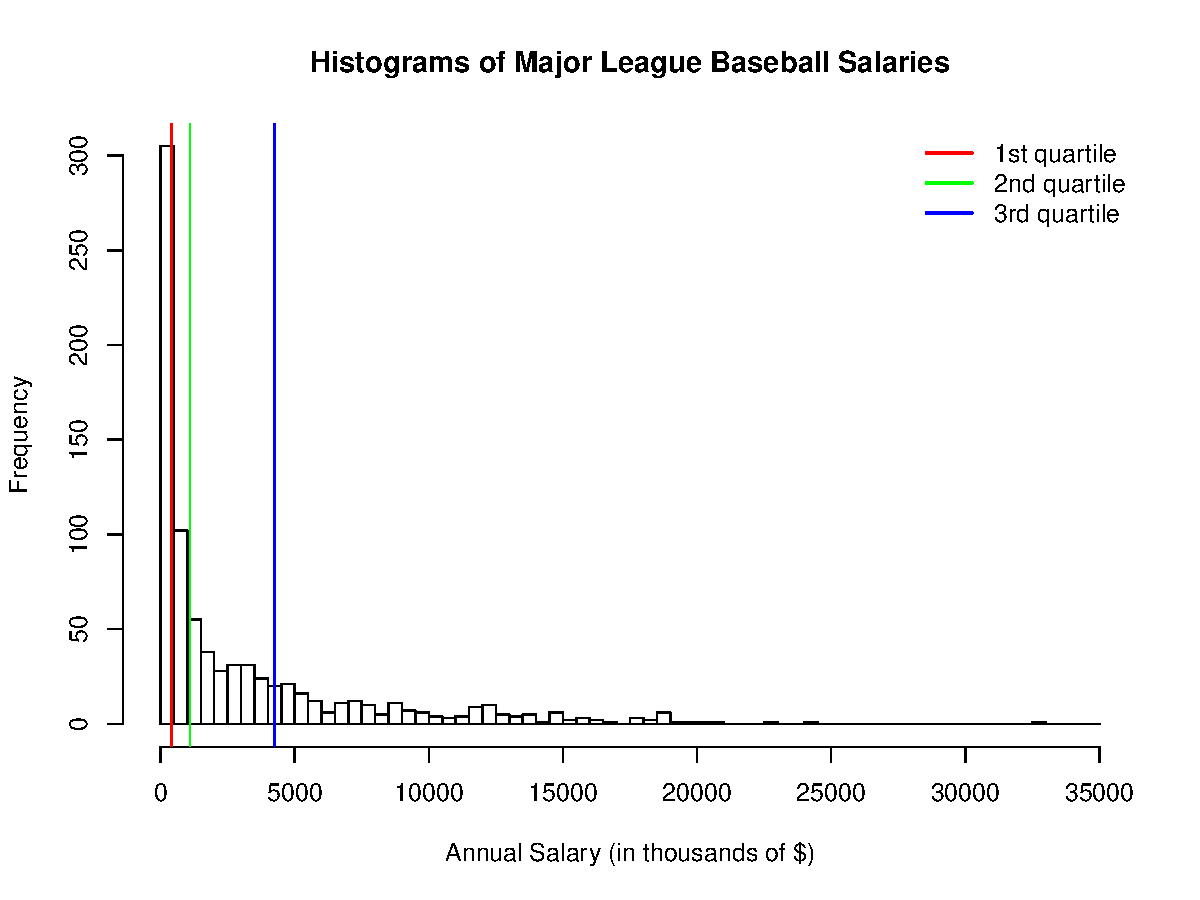
\includegraphics[height=5.5cm]{figure/MLB_quartiles.pdf}
\end{center}

\end{frame}
%-------------------------------------------------------------------------------




%pdf("MLB_quartiles2.pdf", width=8, height=6)
%hist(MLB$salary, breaks=seq(0, 35000, by=500), xlab="Annual Salary (in thousands of $)", main="Histograms of Major League Baseball Salaries", 
%     xlim=c(0,5000))
%abline(v=summary(MLB$salary)[c(2,3,5)], col=c("red", "green", "blue"))
%legend("topright", legend=c("1st quartile", "2nd quartile", "3rd quartile"), 
%       col=c("red", "green", "blue"), lty=c(1,1, 1), lwd=2, bty='n')
%dev.off()
%-------------------------------------------------------------------------------
\begin{frame}[fragile]
\frametitle{MLB Data Quartiles}

\begin{verbatim}
summary(MLB$salary)
   Min. 1st Qu.  Median    Mean 3rd Qu.    Max.
  400.0   418.3  1094.0  3282.0  4250.0 33000.0
\end{verbatim}

\begin{center}
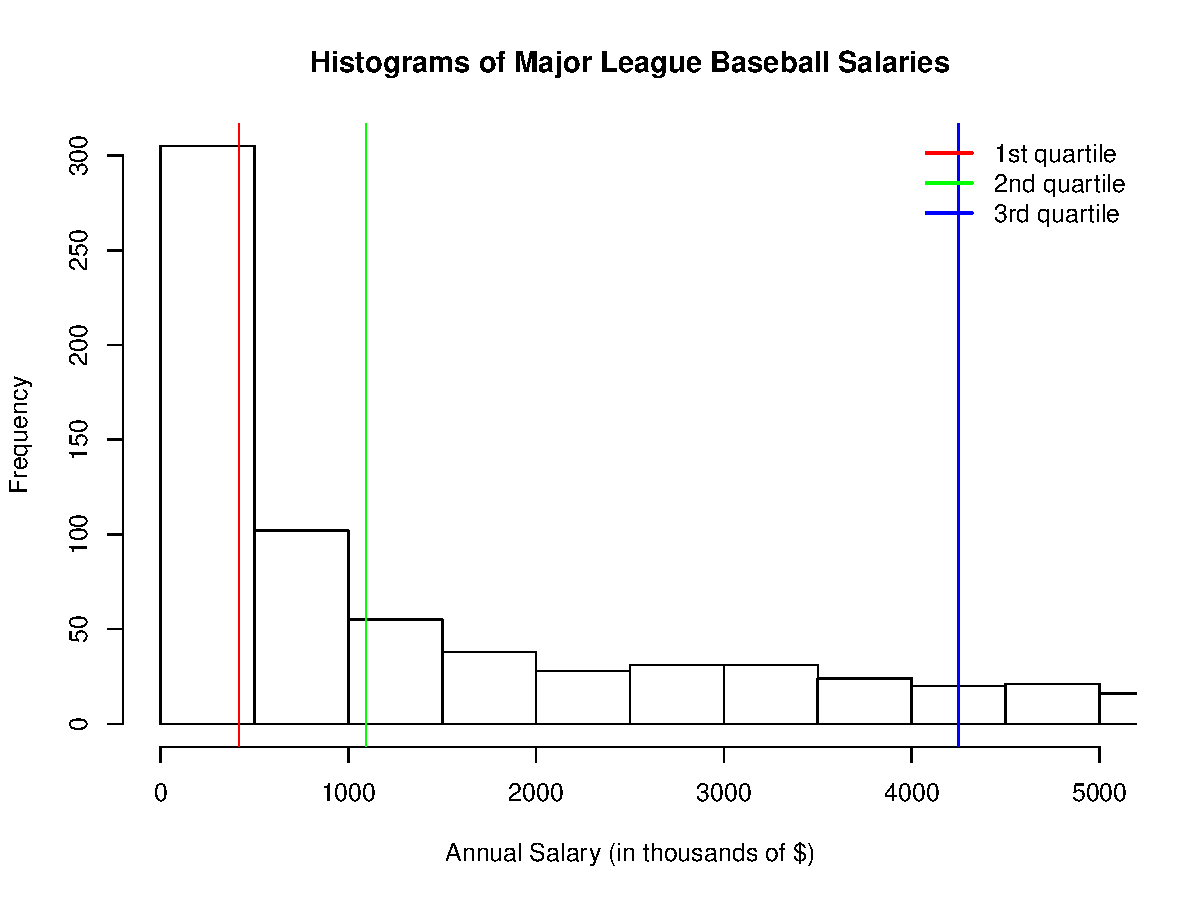
\includegraphics[height=5.5cm]{figure/MLB_quartiles2.pdf}
\end{center}

\end{frame}
%-------------------------------------------------------------------------------



%-------------------------------------------------------------------------------
\begin{frame}
\frametitle{Interquartile Range}
The \blue{interquartile range (IQR)} is another, less-used, measure of the spread of a sample:
\pause\[
\mbox{IQR} = \mbox{upper quartile} - \mbox{lower quartile}
\]

\end{frame}
%-------------------------------------------------------------------------------



%-------------------------------------------------------------------------------
\begin{frame}[fragile]
\frametitle{MLB Data Quartiles}

\begin{verbatim}
summary(MLB$salary)
   Min. 1st Qu.  Median    Mean 3rd Qu.    Max.
  400.0   418.3  1094.0  3282.0  4250.0 33000.0
\end{verbatim}

\begin{center}
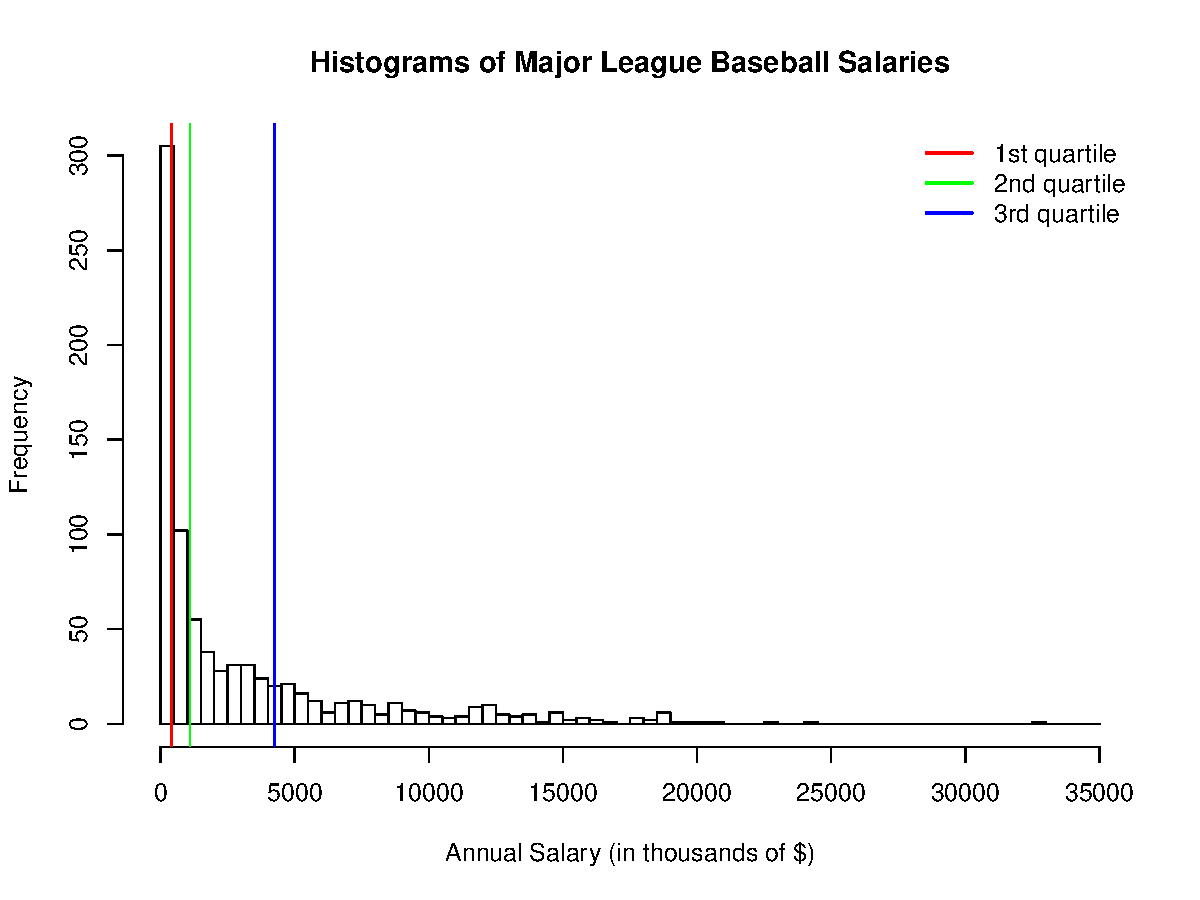
\includegraphics[height=5.5cm]{figure/MLB_quartiles.pdf}
\end{center}

\pause The IQR is (3rd Quartile - 1st Quartile) = 4250.0 - 418.3 = 3831.7\\
i.e the distance between the red and blue line.  


\end{frame}
%-------------------------------------------------------------------------------










%-------------------------------------------------------------------------------
\begin{frame}
\frametitle{Robust Statistics (Chapter 1.6.6)}
\blue{Robust estimates} are statistics where extreme observations (outliers) have less effect on their values, or stated differently:
\begin{itemize}
\pause\item not as sensitive to outliers
\pause\item more ``resistant to outliers''
\end{itemize}

\end{frame}
%-------------------------------------------------------------------------------



%-------------------------------------------------------------------------------
\begin{frame}
\frametitle{Robust Statistics (Chapter 1.6.6)}
One example illustrating the philosophy of ``robustifying'' to outliers is scoring in figure skating: \blue{drop the highest \& lowest scores} and only then take the average.  

\vspace{0.5cm}

\pause Say we have a figure skater who gets judged by judges from countries V-Z. The scores are as follows:
\begin{center}
\begin{tabular}{r||ccccc}
\hline
Country & V & W & X & Y & Z \\ 
\hline
Score & 4.0 & 5.2 & 5.2 & 5.3 & 6.0 \\ 
\hline
\end{tabular}
\end{center}

\vspace{0.5cm}

\pause Drop the 4.0 and 6.0, then the final score is: $\frac{5.2 + 5.2 + 5.3}{3} = 5.23$
\end{frame}
%-------------------------------------------------------------------------------



%-------------------------------------------------------------------------------
\begin{frame}
\frametitle{Median and IQR are Robust Statistics}

The median and IQR are called robust estimates because extreme observations have
little effect on their values.

\vspace{0.5cm}

\pause Say we felt that the highest paid player in baseball, Alex Rodriguez, wasn't \blue{paid enough} at 33 million.  So we increase it to 45 million a season!  Then the median and IQR would not change.  


\end{frame}
%-------------------------------------------------------------------------------





%-------------------------------------------------------------------------------
\begin{frame}
\frametitle{Boxplots}
\blue{Boxplots} are visual summaries of a sample $x_1,\ldots,x_n$ based on five statistics that bring to light unusual values (potential outliers):
\begin{enumerate}
\item lower quartile
\item median
\item upper quartile
\item smallest $x_i$
\item largest $x_i$
\end{enumerate}
\end{frame}
%-------------------------------------------------------------------------------





%-------------------------------------------------------------------------------
\begin{frame}
\frametitle{Boxplots}
Example: \# US Forces casualties in the war in Afghanistan for each month from 2008-2009:  

\vspace{0.5cm}

7, 1, 7, 5, 16, 28, 20, 22, 27, 16, 1, 3, 14, 15, 13, 6, 12, 24, 44, 51, 37, 59, 17, 17


\end{frame}
%-------------------------------------------------------------------------------




%pdf("afghanistan.pdf", width=8, height=4)
%casualties <- c(7, 1, 7, 5, 16, 28, 20, 22, 27, 16, 1, 3, 14, 15, 13, 6, 12, 24, 44, 51, 37, 59, 17, 17)
%boxplot(casualties, horizontal=TRUE, xlab="US Forces casualties in Afghanistan for each month 2008-2009")
%dev.off()
%summary(casualties)
%-------------------------------------------------------------------------------
\begin{frame}[fragile]
\frametitle{Boxplots}
\begin{verbatim}
> summary(casualties)  
Min. 1st Qu.  Median    Mean 3rd Qu.    Max. 
1.00    7.00   16.00   19.25   24.75   59.00 
\end{verbatim}
\begin{center}
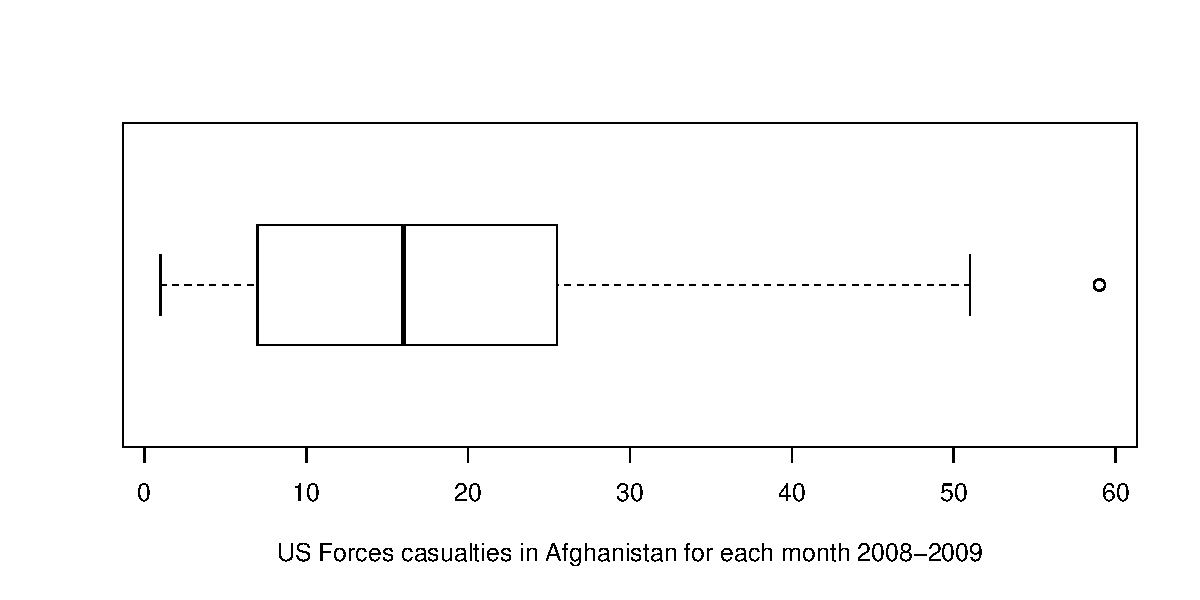
\includegraphics[height=4cm]{figure/afghanistan.pdf}
\end{center}
\pause Please read page 29 on how the determine the length of the \blue{whiskers}: it captures data that is no more than $1.5 \times IQR$ of both ends of the box.  

\end{frame}
%-------------------------------------------------------------------------------



%-------------------------------------------------------------------------------
\begin{frame}
\frametitle{Boxplots to Identify Outliers}
The outlier of 59 corresponds to October 2009, when among other things:
\begin{itemize}
\pause\item On October 3, 2009, a force of 300 Taliban assaulted the American Combat Outpost Keating near the town of Kamdesh of Nuristan province in eastern Afghanistan in the ``Battle of Kamdesh.'' \pause The attack was the bloodiest battle for US forces since the Battle of Wanat in July 2008. The attack resulted in eight Americans killed.
\pause\item 14 died in two separate helicopter crashes on October 26, 2009.
\end{itemize}

\end{frame}
%-------------------------------------------------------------------------------






%-------------------------------------------------------------------------------
\begin{frame}
\frametitle{Outliers Are Relatively Extreme}
An \blue{outlier} is an observation that appears extreme relative to the rest of the data.

\vspace{0.5cm}

\pause Why it is important to look for outliers?  Examination of data for possible outliers serves many useful purposes, including
\begin{itemize}
\pause\item Identifying strong skew in the distribution.
\pause\item Identifying data collection or entry errors.
\pause\item Providing insight into interesting properties of the data.
\end{itemize}

\end{frame}
%-------------------------------------------------------------------------------




%%-------------------------------------------------------------------------------
%\begin{frame}
%\frametitle{Why 1.5 times the IQR?}
%What is the significance of the factor 1.5 when defining what values in a boxplot should be marked as an outlier?  
%\vskip 0.5cm
%\pause Someone asked the creator of the box plot John Tukey ``Why 1.5 times the IQR?''  Tukey's famous response:
%\vskip 0.5cm
%\pause\begin{quotation}
%Because 1 is too small and 2 is too large.
%\end{quotation}
%\end{frame}
%%-------------------------------------------------------------------------------













%------------------------------------------------------------------------------
\begin{frame}[fragile]
\frametitle{Next Time}

We discuss examining/visualizing categorical data.  In particular:

\begin{itemize}
\item Contingency Tables
\item Barplots
\item Piecharts 
\end{itemize}


\end{frame}
%------------------------------------------------------------------------------







\end{document}










